% Source: graduate-coursework/Research/Intro_to_Agents/slides/From_LLMs_to_Multi_Agent_Systems_slides.tex

\documentclass[border=4pt]{standalone}
\usepackage[T1]{fontenc}
\usepackage{graphicx}
\usepackage{tikz}
\usepackage{xcolor}
\usetikzlibrary{arrows.meta,positioning,shapes.geometric,fit,calc,
                decorations.pathreplacing,backgrounds,patterns,trees}

\definecolor{garnet}{HTML}{73000A}
\definecolor{rose}{HTML}{CC2E40}
\definecolor{atlantic}{HTML}{466A9F}
\definecolor{congaree}{HTML}{1F414D}
\definecolor{horseshoe}{HTML}{65780B}
\definecolor{grass}{HTML}{CED318}
\definecolor{honeycomb}{HTML}{A49137}
\definecolor{warmgrey}{HTML}{676156}
\definecolor{sandstorm}{HTML}{FFF2E3}
\definecolor{bk90}{HTML}{363636}
\definecolor{bk70}{HTML}{5C5C5C}
\definecolor{bk50}{HTML}{A2A2A2}
\definecolor{bk30}{HTML}{C7C7C7}
\definecolor{bk10}{HTML}{ECECEC}

\tikzset{
  agentbox/.style={
    rectangle, draw=#1, fill=#1!8, thick,
    minimum width=2.2cm, minimum height=0.8cm,
    font=\small\sffamily, align=center,
    inner sep=4pt
  },
  agentbox/.default=garnet,
  workerbox/.style={
    rectangle, draw=atlantic, fill=atlantic!8, thick,
    minimum width=1.8cm, minimum height=0.7cm,
    font=\small\sffamily, align=center,
    inner sep=3pt
  },
  tierbox/.style={
    rectangle, draw=#1, fill=#1!5, thick,
    minimum width=6.5cm, minimum height=1.0cm,
    font=\small\sffamily, align=center,
    inner sep=4pt
  },
  tierbox/.default=garnet,
  dataarrow/.style={
    -{Stealth[length=5pt]}, thick, color=#1
  },
  dataarrow/.default=bk70,
  brace/.style={
    decorate, decoration={brace, amplitude=6pt, raise=2pt}, thick, color=#1
  },
  brace/.default=bk50,
  labelnode/.style={
    font=\scriptsize\sffamily, color=bk70
  },
  codebox/.style={rectangle, draw=bk70, fill=bk90, text=white,
    font=\ttfamily\small, inner sep=6pt, align=left, text width=#1},
  codebox/.default=6cm,
  sysprompt/.style={rectangle, draw=rose, dashed, fill=rose!5, thick,
    minimum width=2.0cm, minimum height=0.6cm,
    font=\small\sffamily, align=center, inner sep=3pt},
  tooldef/.style={rectangle, draw=atlantic, fill=atlantic!8, thick,
    minimum width=1.8cm, minimum height=0.6cm,
    font=\small\sffamily, align=center, inner sep=3pt},
  wrapperbox/.style={rectangle, draw=garnet, dashed, thick, fill=garnet!3,
    inner sep=8pt},
  pbar/.style={rectangle, draw=#1, fill=#1!30, thick,
    minimum height=0.3cm, font=\scriptsize\sffamily},
  pbar/.default=horseshoe,
  flag/.style={rectangle, draw=rose, fill=rose!15, thick,
    minimum width=0.8cm, minimum height=0.4cm,
    font=\tiny\sffamily\bfseries},
  failbox/.style={rectangle, draw=rose, fill=rose!10, thick,
    font=\small\sffamily, align=center, inner sep=4pt},
}

\begin{document}
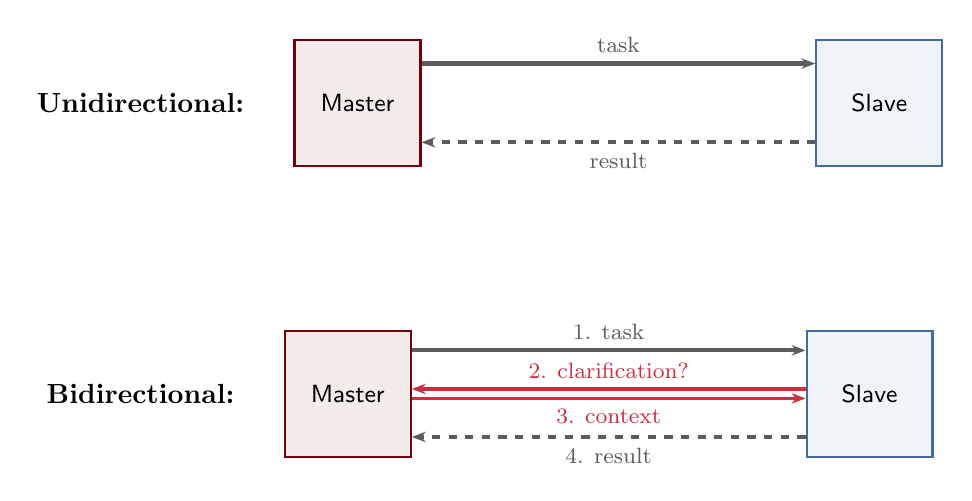
\begin{tikzpicture}[node distance=0.8cm and 1.5cm]
  % Unidirectional
  \node[font=\bfseries, anchor=east] (label1) {Unidirectional:};
  \node[agentbox=garnet, right=0.5cm of label1, minimum width=1.6cm, minimum height=1.6cm] (m1) {Master};
  \node[workerbox, right=5cm of m1, minimum width=1.6cm, minimum height=1.6cm] (w1) {Slave};
  \draw[dataarrow, line width=1.5pt] ([yshift=0.5cm]m1.east) -- node[above] {\footnotesize task} ([yshift=0.5cm]w1.west);
  \draw[dataarrow, dashed, line width=1.5pt] ([yshift=-0.5cm]w1.west) -- node[below] {\footnotesize result} ([yshift=-0.5cm]m1.east);

  % Bidirectional
  \node[font=\bfseries, anchor=east, below=3.2cm of label1] (label2) {Bidirectional:};
  \node[agentbox=garnet, right=0.5cm of label2, minimum width=1.6cm, minimum height=1.6cm] (m2) {Master};
  \node[workerbox, right=5cm of m2, minimum width=1.6cm, minimum height=1.6cm] (w2) {Slave};
  \draw[dataarrow, line width=1.5pt] ([yshift=0.55cm]m2.east) -- node[above] {\footnotesize 1. task} ([yshift=0.55cm]w2.west);
  \draw[dataarrow, dashed, line width=1.5pt] ([yshift=-0.55cm]w2.west) -- node[below] {\footnotesize 4. result} ([yshift=-0.55cm]m2.east);
  \draw[dataarrow=rose, line width=1.2pt] ([yshift=0.06cm]w2.west) -- node[above, pos=0.5] {\footnotesize\color{rose} 2. clarification?} ([yshift=0.06cm]m2.east);
  \draw[dataarrow=rose, line width=1.2pt] ([yshift=-0.06cm]m2.east) -- node[below, pos=0.5] {\footnotesize\color{rose} 3. context} ([yshift=-0.06cm]w2.west);
\end{tikzpicture}
\end{document}
